\chapter{Radiative Transitions on the lattice} \label{chap::radTranLattice}

In this chapter we first introduce radiative transition matrix elements and show how they can be decomposed into kinematic factors, transforming with the symmetries of the vector current, multiplying scalar form factors which encode the dynamics of the transition. On the lattice these matrix elements are encoded in three-point functions which feature a local vector current insertion appearing between mesonic creation and annihilation operators. 

By performing a spectral decomposition of the three-point functions, we will find, in a manner similar to our two point calculation,  that any three-point function in principle contains contributions from all states that have the same quantum numbers as the source and sink operators. Each contribution will propagate through Euclidean time and contribute a factor of $e^{-Et}$ such that for large times only the lightest state survives. In general we will also be interested in the excited state matrix elements, their contributions arising from subleading exponentially damped contributions. We circumvent the problem via the use of `optimal' operators. These optimal operators are constructed as linear combinations of operators within our basis. We will show they do in fact dominantly produce a \emph{single} state, and further, that their use in three-point function allows for the non-perturbative determination of matrix elements featuring \emph{excited states} at both the source and sink.

%%%%%%%%%%%%%%%%%%%%%%%%%%%%%%%%%%%%%%%%%%%%%%%%%%%%%%%%%
%%%%%%%%%%%%%%%%%%%%%%%%%%%%%%%%%%%%%%%%%%%%%%%%%%%%%%%%%
%%%%%%%%%%%%%%%%%%%%%%%%%%%%%%%%%%%%%%%%%%%%%%%%%%%%%%%%%

\section{Form-factors and Transitions \label{sec::formfactor}}

The theoretical object we wish to extract is the matrix element, 
\begin{equation}
\langle h'_{J'}(\vec{p}\,',\lambda')|j^\mu | h_J(\vec{p},\lambda) \rangle, 
\end{equation}
 which describes the vector current transition of a spin-$J$, helicity projection $\lambda$, hadron, $h$, to another spin-$J'$, helicity projection $\lambda'$, hadron ,$h'$. The photon couples to the quark fields \footnote{In this calculation we use a non-physical version of QCD in which there are three as opposed to six flavors. Each quark flavor is tuned to approximately the physical strange quark mass such that there is an exact $SU(3)$ flavor symmetry.} within the hadrons (up to a factor of e) via the vector current, $j^\mu = \frac{2}{3}\bar{u}\gamma^\mu u -\frac{1}{3}\bar{d}\gamma^\mu d -\frac{1}{3}\bar{s}\gamma^\mu s $.  
 
 The matrix elements are related to the helicity amplitude for the process $h\rightarrow h'\gamma$ via the inclusion of the final state photon polarization vector, 
 \begin{equation*}
 \mathcal{M}\Big(h(\vec{p},\lambda)\rightarrow h'(\vec{p}\,',\lambda')\gamma(\vec{q},\lambda_\gamma)\Big) = \epsilon_\mu^*(\vec{q},\lambda_\gamma)\langle h'_{J'}(\vec{p}\,',\lambda')|j^\mu | h_J(\vec{p},\lambda) \rangle.
 \end{equation*}
 where $\vec{q} = \vec{p}\,'-\vec{p}$ and the photon has virtuality $Q^2 = |\vec{q}|^2 - \left( E_{h'}(\vec{p}\,') - E_h(\vec{p})\right)^2$. 
 
 In general one writes the matrix element as a sum over products of kinematic factors, transforming with the symmetries of the current, times an unknown coupling which is a function of the photon virtuality, the form factor. For example when one calculates the form factor of a pseudoscalar meson such as the pion a convenient parameterization of the matrix element is 
\begin{equation*}
\langle \pi^+ (p^\prime) | j^\mu | \pi^+ (p) \rangle = \left( p^\prime + p\right)^\mu F_\pi(Q^2).
\end{equation*}
Here the kinematic factor is $\left( p^\prime + p\right)^\mu$ which transforms under parity in the same way as the matrix element. The careful reader will realize that there is another independent kinematic factor which could appear in the decomposition, namely, $  \left( p^\prime - p\right)^\mu F^{[-]}_\pi(Q^2) $, which also transforms correctly under rotations and parity. This quantity can be eliminated via the constraint imposed from current conservation.

In this analysis we consider formfactors and transitions between meson states of integer angular momentum $J$. Form-factors are accessed via vector current matrix elements in which the current appears sandwiched between meson states  that have been projected onto definite momentum $\vec{p}$ and helicity $\lambda$.  A general parameterization of such a matrix element is 

\begin{equation}
\langle h'_{J'}(\vec{p}\,',\lambda')|j^\mu | h_J(\vec{p},\lambda) \rangle = \sum_i K^\mu_i(J^\prime,\vec{p}\,',\lambda';J,p,\lambda)F_i(Q^2) \label{eqn::genericDecompositionHelicity}
\end{equation}
where $K^{\mu}_i$ is a kinematic factor which transforms in the same way as the matrix element. 
%%%%%%%%%%%%%%%%%%%%%%%%%%%%%%%%%%%%%%%%%%%%%%%%%%%%%%%%%
%%%%%%%%%%%%%%%%%%%%%%%%%%%%%%%%%%%%%%%%%%%%%%%%%%%%%%%%%
%%%%%%%%%%%%%%%%%%%%%%%%%%%%%%%%%%%%%%%%%%%%%%%%%%%%%%%%%
\subsection{Vector current matrix elements} \label{ssec::RadTranLat::Decomp}

We adopt a straightforward approach in which we write down the most general Lorentz covariant and parity invariant decomposition of a vector current matrix element in terms of a number of arbitrary form factors. It is convenient in this approach to use the $z$-component of the spin which is not in general equal to the helicity and which we denote by $r$. The choice of using $j_z$ makes the transformation properties of the polarization tensors simpler, one can derive a similar result using a helicity representation. As an illustrative example we demonstrate the method for a pseudoscalar-vector transition relevant to a process such as $\rho \rightarrow \pi \gamma$.   The most general set of kinematic factors one could write down for such a transition is 

\begin{align*}
\langle P(p^\prime) | j^\mu | V(p,r) \rangle &= A_1(Q^2) \epsilon^\mu(p,r)p_+^\alpha q_\alpha \\
&+A_2(Q^2) p_+^\mu \epsilon_\alpha(p,r)q^\alpha \\
&+A_3(Q^2) q^\mu \epsilon_\alpha(p,r) p_+^\alpha \\
&+B_1(Q^2) \epsilon^{\mu\nu\rho\sigma}\epsilon_\nu(p,r)p_{+\rho}q_\sigma
\end{align*}
In which we have chosen to use the basis $p_+ = p^\prime + p$, and $q = p^\prime -p$ for the momenta. $\epsilon_\alpha(p,r)$ represents a polarization vector for a spin-1 particle with momentum $p$ and spin projection $r$. 

Parity invariance requires that 
\begin{align*}
\langle P(p^\prime) | j^\mu | V(p,r) \rangle &= \langle P(p^\prime) | \mathcal{P}^{-1}\mathcal{P} j^\mu  \mathcal{P}^{-1}\mathcal{P}  | V(p,r) \rangle  \\
&= \left[ \mathcal{P} \right]^\mu_\nu \langle P(-p^\prime) | j^\mu | V(-p,r) \rangle
\end{align*}

Where we have used the fact that under parity our states transform as $\mathcal{P} | P(p,r)\rangle = -|P(-p,r)\rangle $, $\mathcal{P} | V(p,r)\rangle = -|V(-p,r)\rangle $, and $\mathcal{P} j^\mu\mathcal{P}^{-1}  = \left[ \mathcal{P}^{-1} \right]^\mu_\nu j^\nu$ \footnote{  \unexpanded{$ \left[ \mathcal{P}^{-1} \right]^\mu_\nu  = \left[ \mathcal{P} \right]^\mu_\nu  = \mathrm{diag}(+---)$ } } . Using the fact that $\epsilon^\mu(-p,r) = - \left[\mathcal{P}\right]^\mu_\nu \epsilon^\nu(p,r)$ we see that the above decomposition is invariant under parity provided $A_i(Q^2) =0$. 
Current conservation provides an additional constraint on the decomposition, 
\begin{align*} 
&0 = \partial_\mu \langle A(p^\prime,r^\prime) | j^\mu | V(p,r) \rangle \\
\Rightarrow \quad & 0 = q_\mu \langle A(p^\prime,r^\prime) | j^\mu | V(p,r) \rangle
\end{align*}
In this case the kinematic factor vanishes when we dot in the photon momentum, $q_\mu  \epsilon^{\mu\nu\rho\sigma}\epsilon_\nu(p,r)p_{+\rho}q_\sigma = 0$. Using these tools we can build parity invariant Lorentz covariant decompositions of vector current matrix elements for mesons of arbitrary spin at the source and sink. We find 
\begin{align*}
\langle P(p^\prime) | j^\mu | V(p,r) \rangle =B_1(Q^2) \epsilon^{\mu\nu\rho\sigma}\epsilon_\nu(p,r)p_{+\rho}q_\sigma
\end{align*}

More generally there can be more than one form factor occurring in such a decomposition\footnote{For example a vector particle has three form factors.}. In this case there is some ambiguity associated with the decomposition. As a first example we can consider the variables used, for example $p$ and $p^\prime$ are an equally valid set of variables to use in the decomposition (as opposed to our choice of $p_+$ and $q$) but would lead to a different normalization of the form-factor $B_1(Q^2)$. In the case of multiple form factors one is also free to perform a linear transformation on the $K^{\mu}_i$ as $\tilde{K}^\mu_i = L_{ij}K^\mu_j$, which in turn causes a redefinition of the $F_i$. Further in the case that one wants to compare results between two different calculations using different bases it is necessary to construct the mapping, $L$, which in the case of several form-factors becomes algebraically cumbersome.
 
A conventional parameterization for the matrix elements is the Multipole Expansion introduced earlier in \chapref{chap::QM}. For convenience of calculation we work with an arbitrary set of form-factors which we then eliminate in favor of the multipole form-factors where appropriate. This is done in direct analogy with \cite{Durand:1962zza,Dudek:2009kk}.

We now proceed to sketch the derivation\footnote{A more complete description can be found in \cite{Durand:1962zza}}. Defining the vertex function in the Breit frame ($\vec{p} = |p|\hat{z}$ , $\vec{p^\prime} = -\vec{p}$) 
\begin{align*}
\Gamma_{J^\prime\lambda^\prime;J\lambda}^\nu &= \langle J^\prime \lambda^\prime p^\prime | e^{i \pi J_2} j^\nu | J \lambda  p\rangle = \langle J^\prime \lambda^\prime| e^{i\xi_{p^\prime} K_3} e^{i \pi J_2} j^\nu e^{-i\xi_p K_3}  | J \lambda  \rangle
\end{align*}
where the operator $e^{-i\xi_p K_3}$ acting on a rest state effects to boost the state along the $z$-axis to momentum $p\hat{z}$. One can show that this matrix element can be reexpressed as a sum over matrix elements of tensors which transform irreducably under the rotation group -- this is the essence of the multipole decomposition. Each tensor appearing in the decomposition also independently satisfies the Wigner-Eckart Theorem allowing us to solve for the reduced matrix elements which we identify as the various multipole moments of the system. Our construction is identical to Durand's and we refer the reader to \cite{Durand:1962zza} for further details. 

The longitudinal and transverse components\footnote{Here longitudinal refers to the helicity zero polarization state which appears for virtual photons while transverse means the plus/minus helicity projections.} of the vector current transform differently under rotations and one must allow for a different set of reduced matrix elements for each. In the Breit frame the scalar and $z$ component are linked through current conservation as $(E^\prime - E ) \Gamma_{J^\prime\lambda^\prime;J\lambda}^0 = -2p_z \Gamma_{J^\prime\lambda^\prime;J\lambda}^3$ and one can reconstruct the charge moments using only the scalar portion of the vertex function as
\begin{equation}
 \Gamma_{J^\prime\lambda^\prime;J\lambda}^0 = \left(-1\right)^{2J^\prime} \sum_k \begin{pmatrix} 
 J^\prime & k & J \\
 \lambda^\prime & 0 & \lambda 
 \end{pmatrix} \langle J^\prime || T^k_0 || J \rangle  \bigg|_{(-1)^k = \delta P}
\end{equation}
where the variable $\delta P$ is the product of the initial and final parities. A similar expression for the transverse components may be derived, one obtains 

\begin{equation}
 \Gamma_{J^\prime\lambda^\prime;J\lambda}^\pm = \left(-1\right)^{2J^\prime} \sum_{k=1}
  \begin{pmatrix} J^\prime & k & J \\
 \lambda^\prime & \pm 1 & \lambda  \end{pmatrix} 
 \langle J^\prime || T^k_\pm || J \rangle  .
\end{equation}

We note that in the case of identical particles the sum ocurring above is restriced to odd values of $k$. A conventional redefinition of the reduced matrix elements is 
\begin{align*}
 \langle J^\prime || T^k_\pm || J \rangle &= \frac{1}{2}\left[ \left(1 + (-1)^k\delta P\right)E_k + \left(1 - (-1)^k \delta P \right)  M_k  \right] \\
  \langle J^\prime || T^k_0 || J \rangle &= \frac{1}{2} \left(1 + (-1)^k\delta P\right)C_k 
\end{align*} 
where E(M)[C] indicate electric(magnetic)[charge] multipole elements.  

Returning now to our pseudoscalar-vector example we see that $B_1(Q^2)$ can be identified as a magnetic dipole ($M_1$) form factor. More generally there can be multiple form factors occurring in any decomposition, each form factor being a linear combination of the multipoles occurring above. One procedure, which allows for efficient conversion between multipole form factors and some arbitrary basis, is to use the equations above to build a linear system, featuring both sets of formfactors, which can be inverted in order to convert to the multipole basis. 

%%%%%%%%%%%%%%%%%%%%%%%%%%%%%%%%%%%%%%%%%%%%%%%%%%%%%%%%%
%%%%%%%%%%%%%%%%%%%%%%%%%%%%%%%%%%%%%%%%%%%%%%%%%%%%%%%%%
%%%%%%%%%%%%%%%%%%%%%%%%%%%%%%%%%%%%%%%%%%%%%%%%%%%%%%%%%
\subsection{Kinematic Decompositions}

Having introduced the technical machinery used to decompose vector current matrix elements we now turn to the decompositions used in this analysis. In particular we will be interested in extracting form factors a transition matrix elements of pseudoscalar and vector mesons. As mentioned previously the form factor decomposition for a pseudoscalar such as the pion may be written as
\begin{equation} \label{eqn::pion_decomp}
\langle \pi^+ (p^\prime) | j^\mu | \pi^+ (p) \rangle = \left( p^\prime + p\right)^\mu F_\pi(Q^2).
\end{equation}

We will also be interested in transitions between two different pseudoscalar particles. Again there is a single form factor, but here the kinematic factor is different due to the difference in mass between the initial and final states. The decomposition we will use is 
\begin{align}\label{eqn::pipip_decomp}
\big\langle \pi'^+ & (\vec{p}\,') \big| j^\mu \big| \pi^+(\vec{p}) \big\rangle = \left[ (p\!+\!p')^\mu \!+\! \tfrac{m'^2 - m^2}{Q^2} (p' \!-\! p)^\mu \right]\!  F_{\pi'\pi}(Q^2). 
\end{align} 

The transition matrix-element between a vector particle and a pseudoscalar can be expressed as\footnote{Note that here we use a slightly different normalization relative to that presented in \secref{ssec::RadTranLat::Decomp}.}
\begin{align}
\big\langle \pi^+(\vec{p}\,') \big| j^\mu \big| \rho^+(\lambda, \vec{p}) \big\rangle  = \epsilon^{\mu \nu \rho \sigma} p'_\nu\, p^{\,}_\rho \,\epsilon^{\,}_\sigma(\lambda, \vec{p}\,) \, \tfrac{2}{m_\pi + m_\rho} F_{\rho \pi}(Q^2),\label{rho_pi_ff}
\end{align} 
and for a vector meson stable under the strong interactions, the transition form-factor at ${Q^2=0}$ can be related to the radiative decay width ${\Gamma( \rho^+ \to \pi^+ \gamma) = \frac{4}{3} \alpha \frac{\lvert \vec{q}\,  \rvert^3}{(m_\rho + m_\pi)^2} \lvert F_{\rho \pi}(0) \rvert^2    }$, where $\vec{q}$ is the momentum of the final-state photon in the rest-frame of the decaying $\rho$ meson.


A vector particle has three form factors once current conservation, parity invariance, and time reversal invariance are demanded  \cite{Arnold:1979cg}. One basis is 
\begin{align}
\big\langle \rho&^+(\lambda',\vec{p}\,') \big| j^\mu \big| \rho^+(\lambda, \vec{p}) \big\rangle \nonumber \\
= 	&- \big[(p+p')^\mu \; \epsilon^*(\lambda',\vec{p}\,') \cdot \epsilon(\lambda,\vec{p}) \big]\; G_1(Q^2) \nonumber \\
	&+ \big[\epsilon^\mu(\lambda,\vec{p}) \, \epsilon^*(\lambda',\vec{p}\,') \!\cdot\! p + \epsilon^{\mu*}(\lambda',\vec{p}\,')\, \epsilon(\lambda,\vec{p})\!\cdot\! p' \big]\, G_2(Q^2) \nonumber \\
	&- \big[(p+p')^\mu \; \epsilon^*(\lambda',\vec{p}\,') \!\cdot\! p \;  \epsilon(\lambda,\vec{p})\!\cdot\! p' \, \tfrac{1}{2m^2} \big]\; G_3(Q^2), \label{eqn::rho_Gi_basis}
\end{align} 
with a corresponding set of three independent dimensionless form-factors $G_1$, $G_2$, $G_3$. A convenient basis having a clearer physical motivation is provided by the expansion of the vector current in terms of multipoles \cite{Durand:1962zza}, which in this case leads to a set of form-factors,
\begin{align}
G_C &= \left(1 + \tfrac{Q^2}{6m^2} \right) G_1 - \tfrac{Q^2}{6m^2} \, G_2 + \tfrac{Q^2}{6m^2} \left(1 + \tfrac{Q^2}{4m^2} \right) G_3 \nonumber \\
G_M &= G_2 \nonumber \\
G_Q &= G_1 - G_2 + \left(1 + \tfrac{Q^2}{4m^2} \right) G_3, \label{eqn::rho_Gmultipole_basis}
\end{align}
which are proportional to the charge ($C_0$), magnetic dipole ($M_1$), and quadrupole ($C_2$) multipoles respectively. At $Q^2=0$ they are related to the charge, magnetic moment and quadrupole moment of the vector meson: $G_C(0) = 1$, $G_M(0) = 2 m\cdot  \mu_\rho$, $G_Q(0) = m^2 \cdot Q_\rho$.

The other form-factors we considered above may also be identified with a particular multipolarity -- in the ${\rho \to \pi \gamma}$ transition case the single form-factor is of magnetic dipole ($M_1$) type, while for the $\pi$ cases it is a charge form-factor  $(C_0)$. The form factors we extract are real functions of $Q^2$. 

%%%%%%%%%%%%%%%%%%%%%%%%%%%%%%%%%%%%%%%%%%%%%%%%%%%%%%%%%
%%%%%%%%%%%%%%%%%%%%%%%%%%%%%%%%%%%%%%%%%%%%%%%%%%%%%%%%%
%%%%%%%%%%%%%%%%%%%%%%%%%%%%%%%%%%%%%%%%%%%%%%%%%%%%%%%%%

\section{Three Point Functions} \label{sec::3ptFun}
Now that we have introduced the objects of interest, vector current matrix elements, and shown how they can be decomposed into form factors encoding the dynamics of hadronic transitions, we can proceed to illustrate how one can apply the machinery of lattice QCD to extract the matrix elements of interest from three-point correlation functions. The essential structure of the correlation functions of interest is 
\begin{equation}
C_{f\mu i}(\Delta t, t) = \langle 0 | \mathcal{O}_f(\Delta t) j_\mu(t) \mathcal{O}_i^\dagger(0) | 0 \rangle. 
\end{equation}
Here the operators, $\mathcal{O}_{f,i}$, are capable of interpolating the mesonic states of interest from the vacuum. Insertion of a complete set of states and performing time evolution of the operators yields, in a manner similar to that presented in \secref{sec::Spec:corrFunc}, a spectral decomposition, 
\begin{align}
C_{f\mu i}(\Delta t, t) = \sum_{\mathfrak{n}_f,\mathfrak{m}_i} \frac{1}{2E_{\mathfrak{n}_f}}\frac{1}{2E_{\mathfrak{m}_i}}e^{-E_{\mathfrak{n}_f}(\Delta t -t)} e^{-E_{\mathfrak{m}_i}t}  \langle 0 | \mathcal{O}_f(0) | \mathfrak{n}_f \rangle \, \langle \mathfrak{n}_f |  j_\mu(0)  | \mathfrak{m}_i \rangle \, \langle \mathfrak{m}_i | \mathcal{O}_i^\dagger(0) | 0 \rangle. 
\end{align}
In this manner we see that the three-point correlation function encodes the matrix element of interest, $ \langle \mathfrak{n}_f |  j_\mu(0)  | \mathfrak{m}_i \rangle$, as well as \emph{all} other transition matrix elements having the same quantum numbers as the source and sink operators. 

Our job now is to determine how we can extract a \emph{single} matrix element from such a correlation function. The summation above runs over all states, but clearly, if the separation between operators is large, $\Delta t >> t >> 0 $, we see that the correlation function will become dominated by the lightest states in the $i$ and $f$ channels. At more modest separations we expect there to be subleading, exponentially suppressed, `pollution' terms which could potentially be a source of systematic error in a calculation interested only in ground state matrix elements. One general feature, present in lattice calculations, is that statistical noise tends to increase with increasing operator separation -- the naive approach of simply pulling the source and sink far apart may not be practical in explicit calculation. 

For our purposes we are also interested in extraction of \emph{excited} state matrix elements whose contribution to the above correlation function is exponentially suppressed. In principle one could attempt to determine the value of these matrix elements via their time dependence but the resolution of such subleading, exponentially suppressed signals proves troublesome in practice.  

%%%%%%%%%%%%%%%%%%%%%%%%%%%%%%%%%%%%%%%%%%%%%%%%%%%%%%%%%
%%%%%%%%%%%%%%%%%%%%%%%%%%%%%%%%%%%%%%%%%%%%%%%%%%%%%%%%%
%%%%%%%%%%%%%%%%%%%%%%%%%%%%%%%%%%%%%%%%%%%%%%%%%%%%%%%%%

\subsection{Optimized Operators} \label{sec::OptOps}

Our solution to this problem is to generate `optimal' operators which dominantly create only a single state in the spectrum. In general a color-singlet operator $\mathcal{O}_i^\dag$ having definite $J^{PC}$ can produce all QCD eigenstates having those quantum numbers,
\begin{equation}
	\mathcal{O}_i^\dag |0\rangle = \sum_\mathfrak{n} \frac{1}{2E_{\mathfrak{n}}} |\mathfrak{n} \rangle \langle \mathfrak{n} | \mathcal{O}_i^\dag |0\rangle.  \nonumber
\end{equation}
We seek to determine optimized interpolators, $\Omega_\estate{n}^\dagger$, which when acting on the vacuum strongly interpolate only a \emph{single} state with much reduced contributions from other states,
\begin{align*}
\Omega_\estate{n}^\dagger | 0 \rangle &= \frac{1}{2E_{\mathfrak{n}}}|\estate{n}\rangle \langle \estate{n} | \Omega^\dagger_\estate{n} | 0 \rangle + \sum_{\estate{m} \neq \estate{n}} \frac{1}{2E_{\mathfrak{m}}}  |\estate{m}\rangle \langle \estate{m} | \Omega^\dagger_\estate{n} | 0 \rangle \\
&=\frac{1}{2E_{\mathfrak{n}}} |\estate{n}\rangle \langle \estate{n} | \Omega^\dagger_\estate{n} | 0 \rangle + \sum_{\estate{m} \neq \estate{n}}  |\estate{m}\rangle \varepsilon_\estate{m}.
\end{align*}
In essence we seek a procedure by which we can minimize the $\varepsilon_\estate{m}$ ($\estate{m} \neq \estate{n}$) relative to the strength with which our operator creates the $\estate{n}$'th state, $\langle \estate{n} | \Omega^\dagger_\estate{n} | 0 \rangle/2E_{\estate{n}}$. 

We will define these optimal operators to be linear combinations of operators within a variational basis. That is operators of generic structure
\begin{equation*}
\Omega_\estate{n}^\dagger = \sum_i w_i^{(\estate{n})} \mathcal{O}_i^\dagger.
\end{equation*}
Returning for a moment to the variational analysis presented in \chapref{chap::Spectroscopy}, we alluded to the fact that the generalized eigenvalue problem we solve, $C(t)v^{(\estate{n})}(t) = \lambda_{\estate{n}}(t) C(t_0) v^{(\estate{n})}(t)$, arises in the context of a variational optimization of the amplitude to create the $\estate{n}$'th state. In the same manner, the best estimate, in a variational sense, for the weights $w_i^{(\estate{n})}$, are the generalized eigenvectors occurring in the generalized eigenvalue problem. We define the optimized operators as 
\begin{equation*}
\Omega_\estate{n}^\dagger = \sqrt{2E_{\estate{n}}}e^{-E_{\estate{n}}t_0/2} \sum_i v_i^{(\estate{n})} \mathcal{O}_i^\dagger,
\end{equation*}
where the coefficient appearing in front of the sum is chosen to give the normalization $\langle \estate{n}| \Omega_\estate{n}^\dagger | 0 \rangle = 2E_{\estate{n}}$. In practice we use the \emph{mean} value of $v_i^{(\estate{n})}$ over the ensemble of gauge configurations to generate the weights. This procedure, of solving the generalized eigenvalue problem in a basis of variational interpolating fields and using the generalized eigenvectors to construct optimal operators, is repeated independently for each quantum number and momentum projection that we will use. 

In order to motivate the use of projected operators we first demonstrate their efficacy in projecting a single state out of a two point correlation function. In \figref{fig::TwoPointRelax} we plot the two point function $\langle 0 | \mathcal{O}(t) \mathcal{O}^\dagger(0) | 0 \rangle$ for $\mathcal{O} = \bar{\psi}\gamma_5\psi, \Omega_\pi$, where the data have been normalized such that they `flatten' to a value of one once the pion dominates the correlation function\footnote{$\bar{\psi}\gamma_5\psi$ is one of the simplest local fermion bilinears that is capable of producing a pion.}. We find that the optimized operator is capable of isolating the pion at significantly earlier times than the fermion bilinear $\bar{\psi}\gamma_5\psi$. 

\afterpage{
\begin{figure}[htbp]
\begin{centering}
\includegraphics[width=0.8\linewidth]{figures/radTrans/TwoPointRelaxation.pdf}
\caption{ Rest frame pion correlator using $\bar{\psi}\gamma_5\psi$ (red) as compared to the optimized operator $\Omega_0$ in blue. We plot $2m_\pi e^{m_\pi t} \langle 0 | \mathcal{O}(t) \mathcal{O^\dagger}(0) | 0 \rangle / | \langle 0 | \mathcal{O} |\pi\rangle | ^2$ \label{fig::TwoPointRelax}}
\end{centering}
\end{figure}
\clearpage
}

In this manner optimized operators can be used to make the calculation of ground state matrix elements more efficient. As mentioned perviously, we aim to move beyond ground state matrix elements. In order to demonstrate the efficacy of our optimized operators, applied to \emph{excited} states, we plot the \emph{effective mass}\footnote{Denoting the two point function $C(t)$, the effective mass is $-\frac{d}{dt} \ln(C(t))$, which is a constant, specifically the mass, provided a single state dominates the two point function, $C(t)\sim Ae^{-mt}$. The derivative is approximated using a forward finite difference derivative.} for the lightest four states in the $A_2^+$ irrep of momentum direction $\vec{p} = \frac{2\pi}{L}[1,0,0]$\footnote{From this point forward we will adopt the convention that we describe momentum using a directional vector of integers, $\vec{n}_{\vec{p}}$, where the momentum is specified via $\vec{p} = \frac{2\pi}{L}\vec{n}_{\vec{p}}$.}.  

\afterpage{
\begin{figure}
\begin{centering}
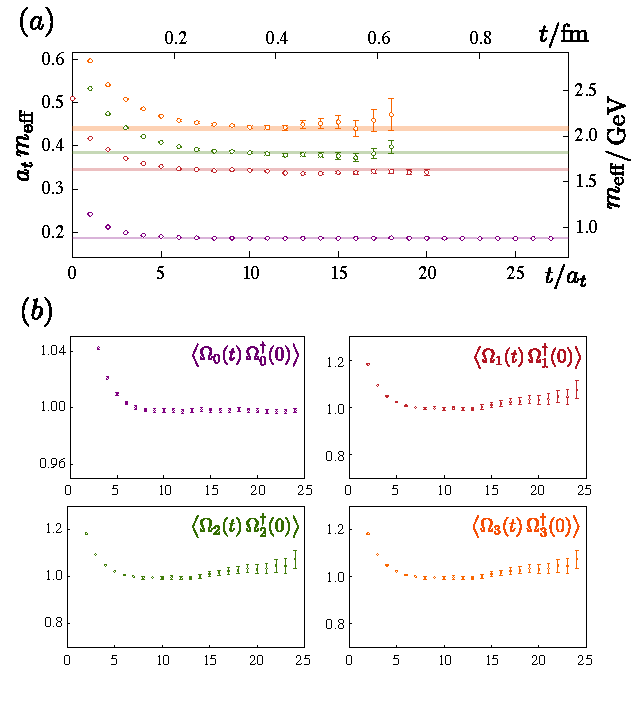
\includegraphics[width=0.8\linewidth]{figures/radTrans/PrinCorr_Eff_D4A2M_mom1.pdf}
\caption{(a) Effective masses of principal correlators for four lightest states in the $A_2^+$ irrep for momentum direction $\vec{n}_{\vec{p}} = [1,0,0]$ along with the energy determined from a two exponential fit. (b) `Optimized' operator correlation functions, $(2E_\mathfrak{n})^{-1} e^{E_\mathfrak{n}t} \big\langle \Omega_\mathfrak{n}(t) \, \Omega_\mathfrak{n}^\dag(0) \big\rangle$, for the four states shown above.\label{fig::SpecD4A2M}}
\end{centering}
\end{figure}
\clearpage
}

%%%%%%%%%%%%%%%%%%%%%%%%%%%%%%%%%%%%%%%%%%%%%%%%%%%%%%%%%
%%%%%%%%%%%%%%%%%%%%%%%%%%%%%%%%%%%%%%%%%%%%%%%%%%%%%%%%%
%%%%%%%%%%%%%%%%%%%%%%%%%%%%%%%%%%%%%%%%%%%%%%%%%%%%%%%%%

\subsection{Three-Point Functions Using Optimized Operators} \label{sec::OptOps}
Turning first to the case of three-point functions with pion-like operators at the source and sink, we plot in \figref{fig::ThreePointRelaxationPion} the form-factor (as defined in \eqnref{eqn::pion_decomp}) extracted from the three-point function, 
\begin{equation*}
\langle 0 | \mathcal{O}_\pi(\Delta t,\vec{p}_f) j^\mu(t, \vec{q}) \mathcal{O}^\dagger_\pi(0,\vec{p}_i) | 0 \rangle
\end{equation*}
where $\mathcal{O}_\pi$ represents either $\bar{\psi}\gamma_5\psi$ (in red) or the optimized operator $\Omega_\pi$ (in blue). The sink operator, located at $\Delta t = 28\, a_t \sim 0.9 \;\mathrm{fm}$, is in the $\Lambda^C = A_2^+$ irrep of momentum $\vec{n}_{\vec{p}_f} = [1,0,0]$, while the source operator, located at $t = 0$, is at rest in the $\Lambda^{PC} = A_1^{-+}$ irrep. We clearly observe that the optimized operators give rise to a signal which is flat over a number of timeslices away from the source and sink, corresponding to the contribution of just the ground-state pion, while the simpler $\bar{\psi}\gamma_5\psi$ operators over this time range always retain a non-negligible pollution from excited states. Such behavior is expected from our two-point function analysis: for example, at rest we find $\left| \tfrac{ \langle 0 | \bar{\psi}\gamma_5 \psi | \mathfrak{n} = 1\rangle}{  \langle 0 | \bar{\psi}\gamma_5 \psi | \mathfrak{n} = 0\rangle} \right| \sim 0.73$, so the distillation smeared operator $\left[ \bar{\psi} \gamma_5 \psi \right]^\dagger $, acting on the vacuum, creates both the ground and first excited state with comparable strength.

Our principal motivation for using optimized operators is to get access to transitions involving excited states. \figref{rhopiproj} we show matrix elements extracted from three-point correlation functions computed using either the ground-state $\pi$ or first-excited state $\pi'$ optimized operator at the source ($t_i=0,\, \vec{p}_i=[\text{-}1, 0, \text{-}1]$) and either the ground-state $\rho$ or first-excited state $\rho'$ operator at the sink ($t_f = 20\,a_t,\, \vec{p}_f=[1, 0, \text{-}1]$). We observe that there are clear statistically significant signals for excited-state transitions when using the appropriate optimized operators.

%%%%%%%%%%%% OPTIMIZED VERSUS STANDARD OPS %%%%%%%%%%%%%%%%%%%%
\afterpage{
\begin{figure}[htbp]
\begin{centering}
\includegraphics[width=0.8\linewidth]{figures/radTrans/ThreePointRelaxationPion.pdf}
\caption{Form-factor from vector current three-point function with pion operators at source ($t=0$, $\vec{n}=[0,0,0]$) and sink ($\Delta t = 28\,a_t$, $\vec{n} = [1,0,0]$). Red points correspond to using the `unoptimized' bilinear $\bar{\psi} \gamma_5 \psi$;  the `optimized' operator is shown in blue. \label{fig::ThreePointRelaxationPion}}
\end{centering}
\end{figure}
\clearpage
}

%%%%%%%%%%%% OPTIMIZED GROUND STATES & EXCITED %%%%%%%%%%%%%%%%%%%%
\afterpage{
\begin{figure}[htbp]
\begin{centering}
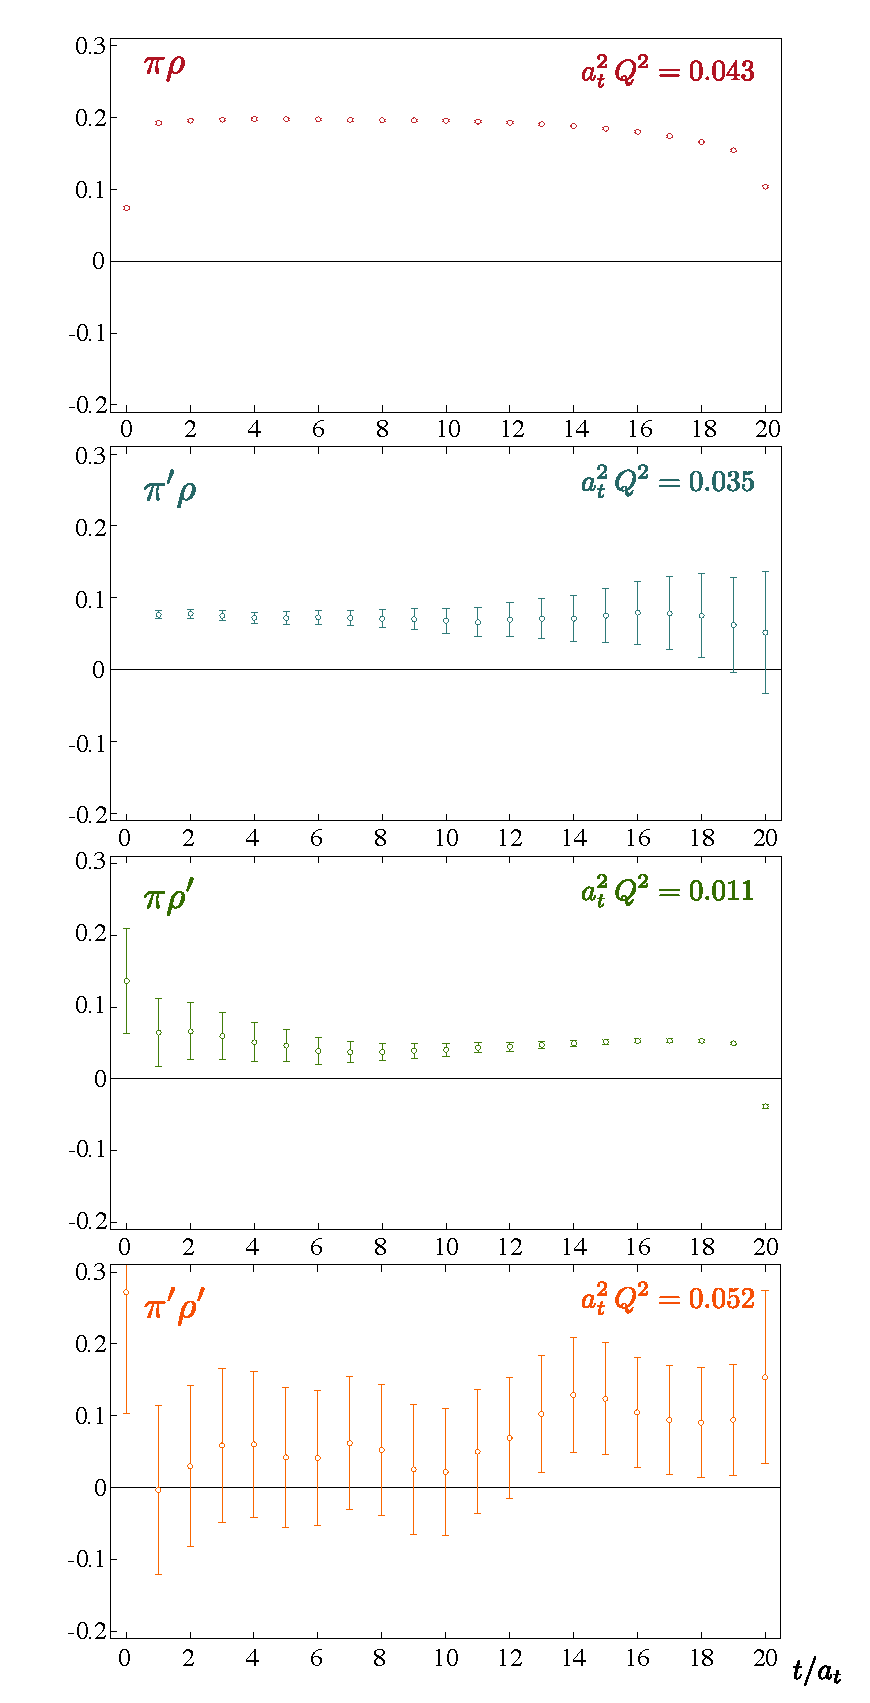
\includegraphics[width=0.5\linewidth]{figures/radTrans/ThreePointProjection.pdf}
\caption{ Form-factors extracted from optimized three-point correlation functions with a $\pi$ or $\pi'$ operator with ${\vec{p}=[\text{-}1,0,\text{-}1]}$ at $t=0$ and a $\rho$ or $\rho'$ operator with ${\vec{p}=[1,0,\text{-}1]}$ at $t= 20\,a_t$. The source-sink separation in physical units is roughly 
0.7 fm. \label{rhopiproj}}\end{centering}
\end{figure}
\clearpage
}

%%%%%%%%%%%% DEPENDENCE ON DELTA-T AND FITTING %%%%%%%%%%%%%%%%%%%%
\afterpage{
\begin{figure}[htbp]
\begin{centering}
\includegraphics[width=\linewidth]{figures/radTrans/Fpi_src_snk_separation_combined.pdf}
\caption{ Upper panel shows the pion ground-state form-factor extracted from correlation functions with source-sink separations of $\Delta t = (12,16,28)\, a_t$ using the procedure of fitting with \eqnref{three_point_fit}. The lower panel illustrates this using the example of $\vec{n}_{\vec{p}_i} = [1,0,0],\, \vec{n}_{\vec{p}_f} = [2,0,0]$.\label{fig::ThreePointSourceSinkSeparation}  }
\end{centering}
\end{figure}
\clearpage
}

In general, even for optimized operators, there may still be some residual contamination coming from states that lie beyond the reach of our variational basis, and indeed curvature away from flat behavior as we approach the source or sink timeslice is observed in Figures~\ref{fig::ThreePointRelaxationPion} and \ref{rhopiproj}. 

In order to make maximal use of the time-series data, in particular in those regions where there remains some unwanted excited-state contribution, we opt to perform a correlated fit over a time range with the form,
\begin{equation}
F(Q^2; t) =  F(Q^2)  + f_f \, e^{-\delta E_{f}\,(\Delta t - t)} + f_{i} \,  e^{- \delta E_i\, t} 
\label{three_point_fit}
\end{equation}
where $f_f, \delta E_f, f_i, \delta E_i$ and $F(Q^2)$ are real fit parameters. We make further use only of the constant term, which corresponds to the desired form-factor. Fitting the data to this form also exposes the energy scale of the pollution terms, $\delta E_f$ and $\delta E_i$. Generically, when present, we find that these energies lie at or above the scale of the largest energies we reliably extract in our two-point function variational analysis. In cases where there is a clear extended plateau region, we may exclude the exponential terms and perform a fit to a constant value.


We demonstrate the viability of our fitting method in \figref{fig::ThreePointSourceSinkSeparation}. A visible plateau is only observed for $\Delta t = 28\, a_t$, while for $\Delta t = 12\, a_t, 16\, a_t$, we make use of a fit using \eqnref{three_point_fit}, extracting compatible values for the form factor even in the face of significant amounts of pollution. The upper panel shows that this procedure is generally applicable and leads to form-factors from each time-separation that are in agreement across a range of $Q^2$ -- additional values of $\Delta t$ were also explored with similar results.

In practice, while we extract a very large number of form-factor determinations at many $Q^2$-values, we choose to make use of only those where application of \eqnref{three_point_fit} to $F(Q^2;t)$ shows modest excited-state contributions. Any cases where a clear trend toward a constant value is not visible are discarded.

%%%%%%%%%%%%%%%%%%%%%%%%%%%%%%%%%%%%%%%%%%%%%%%%%%%%%%%%%
%%%%%%%%%%%%%%%%%%%%%%%%%%%%%%%%%%%%%%%%%%%%%%%%%%%%%%%%%
%%%%%%%%%%%%%%%%%%%%%%%%%%%%%%%%%%%%%%%%%%%%%%%%%%%%%%%%%

\subsection{Extracting Form Factors} \label{sec::FFExtract}
In \eqnref{eqn::genericDecompositionHelicity} we present the most general form of the decomposition of a vector current matrix element into independent form factors, $F_i(Q^2)$, multiplying their associated kinematic factors, $K_i^\mu$, which are functions of the momentum, spin, and helicity projection. Moving, for the moment, to an exhaustive notation, we see that we can decompose a three-point correlation function featuring \emph{optimized} operators as 
\begin{align}
\langle 0 | \Omega_{\estate{n}_f,\vec{p}_f, \lambda_f}(\Delta t) &j^\mu_{\vec{q}}(t) \Omega^\dagger_{\estate{n}_i,\vec{p}_i, \lambda_i}(0) | 0 \rangle \notag \\ &= e^{-E_{\estate{n}_f}(\Delta t - t)} e^{-E_{\estate{n}_i}t} \langle \estate{n}_f ,\vec{p}_f, \lambda_f | j^\mu | \estate{n}_i,\vec{p}_i, \lambda_i \rangle + \ldots \label{eqn::llsq_p}\\ 
&=  e^{-E_{\estate{n}_f}(\Delta t - t)} e^{-E_{\estate{n}_i}t} \sum_j K^\mu_j(\estate{n}_f ,\vec{p}_f, \lambda_f;\estate{n}_i,\vec{p}_i, \lambda_i ) F_j(Q^2) + \ldots \notag,
\end{align}
where the ellipses represent suppressed contributions from states other than ($|\estate{n}_f\rangle , |\estate{n}_i\rangle $), which have been shown in the preceding subsection to be small. 

In general \eqnref{eqn::llsq_p} represents an under-determined linear system. This is to say that on the l.h.s. we have a single matrix element while on the right there are multiple form factors appearing which must be disentangled. We choose to build a constrained or over-constrained linear system featuring many such equations, each occurring at the same $Q^2$, which we then invert to obtain the form factors, $F_j(Q^2)$. Fixing the state choices, $\estate{n}_{f,i}$, using the indexing $a = \left(\vec{p}_f, \lambda_f;\mu;\vec{p}_i \lambda_i\right)$, and removing the time dependence we can rewrite the above equation as 
\begin{align}
\Gamma_a(\Delta t, t) &= e^{E_{\estate{n}_f}(\Delta t - t)} e^{E_{\estate{n}_i}t} \langle 0 | \Omega_{\estate{n}_f,\vec{p}_f, \lambda_f}(\Delta t) j^\mu_{\vec{q}}(t) \Omega^\dagger_{\estate{n}_i,\vec{p}_i, \lambda_i}(0) | 0 \rangle \notag \\
&= \sum_jK_j(a)F_j(Q^2) + \ldots.
\end{align}
In this manner we exploit the redundancy of form factors appearing for different current components and helicity combinations. We also, in some cases, average over kinematically equivalent momenta. 

The linear system we solve is $\mathbb{\Gamma} = \mathbb{K} \cdot \mathbb{F}$. Here $\mathbb{\Gamma}$ is a vector over the index $a$, each element $\Gamma_a(\Delta t,t)$, $\mathbb{K}$ a matrix over kinematic factors with indices $a$ and $j$, and $\mathbb{F}$ a vector of form factors indexed by $j$.  A general formulation of such a linear system need not be square, indeed in practice we build over-constrained rectangular linear systems. The system can be converted into a square system: $\mathbb{K}^\dagger \mathbb{\Gamma} = \left[ \mathbb{K}^\dagger \mathbb{K} \right ] \mathbb{F}$, which we invert using SVD\footnote{In the case where only a single form factor contributes this method of solution reduces to computing an average.}. 


%%%%%%%%%%%%%%%%%%%%%%%%%%%%%%%%%%%%%%%%%%%%%%%%%%%%%%%%%
%%%%%%%%%%%%%%%%%%%%%%%%%%%%%%%%%%%%%%%%%%%%%%%%%%%%%%%%%
%%%%%%%%%%%%%%%%%%%%%%%%%%%%%%%%%%%%%%%%%%%%%%%%%%%%%%%%%

\subsection{Cubic Symmetry} \label{sec::CubSym}
Implicit in the previous sections were a number of assumptions about the nature of states we see in our lattice calculation. Specifically we took advantage of Lorentz symmetry (by assuming we could relate various components of the current to one another) and the organization of hadrons into irreducible representations of the continuous rotation group labeled by an integer $J$ (in the construction of kinematic decompositions) -- neither of these are explicitly good symmetries on the lattice.  

The \emph{cubic} grid, on which we run simulations, is only invariant under cubic rotations, a subset of all rotations, and as such there are different irreps (as discussed in \secref{Spec::Subduce}). To correctly reflect the symmetry of our theory then, we should label our correlation functions according to irreducible representations of the cubic symmetry. In practice this is what we do by computing using the subduced operators introduced in \secref{sec::OptOps}. Using these operators, the three-point functions take the form,
\begin{equation}
	\big\langle 0 \big| \Omega_{\mathfrak{n}_\mathrm{f}, \vec{p}_\mathrm{f}}^{\Lambda_\mathrm{f},\mu_\mathrm{f}}(\Delta t) \, j_{\vec{q}}^{\Lambda_\gamma, \mu_\gamma}(t) \, \Omega_{\mathfrak{n}_\mathrm{i}, \vec{p}_\mathrm{i}}^{\Lambda_\mathrm{i},\mu_\mathrm{i}\dag}(0) \big| 0 \big\rangle, \label{subduced_3pt}
\end{equation}
where the indices $\Lambda$, $\mu$ label the cubic group irrep and the `row' ($1\cdots\text{dim}(\Lambda)$) of the irrep. 

As explained in \secref{Spec::Cubic} it \emph{may} be the case that there are underlying continuum-like symmetries which emerge when the mesh becomes sufficiently fine.  It would be irresponsible to use this putative symmetry without first demonstrating its realization in explicit calculation\footnote{The linear system, as presented, would also not be satisfactorily solvable if the symmetry were not present.}. 

\afterpage{
\begin{sidewaysfigure}[htbp]
\begin{center}
\includegraphics[width=\linewidth]{figures/radTrans/RotationalSymmetryRestoration.pdf}
\end{center}
\caption{Left: We plot the mass spectrum for the lowest $J^{PC} = 1^{--}, 1^{+-}$ states projected onto momentum $\vec{n}_{\vec{p}} = [110]$ across the $\Lambda^C = A_1^-,B_1^-,B_2^-,A_2^-$ little group irreps observing degeneracy patterns corresponding to the $\rho$ and $b_1$ mesons. Right: Transition form-factors extracted from the three point function $\langle 0 | \Omega_\rho(28,\vec{p}\;') j^\mu(t,\vec{q}) \Omega_\pi^\dagger(0,\vec{p}) | 0 \rangle$ with  $\vec{n}_{\vec{p}\;'} = [0,1,1]$, $\vec{n}_{\vec{p}} = [0,\text{-1},1]$, and $\vec{n}_{\vec{q}}  = [0,2,0]$.  Observation of consistent form-factor values indicates that we are resolving the different helicity components of a $1^{--}$ meson.  \label{fig::RotSymRest}}
\end{sidewaysfigure}
\clearpage
}

As a primer we first consider the left panel of \figref{fig::RotSymRest} where we show an example of the extracted spectrum across little-group irreps, $\Lambda^C = A_1^-, B_1^-, B_2^-, A_2^-$ for $n_{\vec{p}}=[110]$, where the distribution of states matches the expected subduction patterns for two meson states, a lighter $\rho$ ($J^{PC}=1^{--}$) state and a heavier $b_1$ ($J^{PC}=1^{+-}$) state.

In order to investigate if the lower pattern really does correspond to the different helicity projections of a $J^{PC} =1^{--}$ state we form the optimized `$\rho$' operator  in each of the $A_1^-, B_1^-, B_2^-$ irreps. We then compute the three-point function, 
\begin{equation*}
\langle 0 | \Omega_\rho(\Delta t,\vec{p}\,')\,  j^\mu(t,\vec{q}\,) \,  \Omega_\pi^\dagger(0,\vec{p}\,) | 0 \rangle,
\end{equation*}
for $\vec{n}_{\vec{p}\,'} = [0,1,1]$, $\vec{n}_{\vec{p}} = [0,\text{-}1,1]$, and $\vec{n}_{\vec{q}} = [0,2,0]$. The source operator is the optimized operator for the ground-state pion in the $A_2^+$ irrep. The three different sink irrep choices correspond to the subduced versions of the three helicity projections of a vector meson. For $\Delta t = 28\,  a_t$, the resulting form-factor is plotted in \figref{fig::RotSymRest}, where we observe that while the amount of excited state pollution differs slightly in each irrep, the form-factor values are consistent, indicating that we are observing components of the same $1^{--}$ meson in the three irreps. 

We expect to see a comparable restoration of the rotational symmetry across this calculation, we do not attempt to build decompositions according to the symmetries of the cube, rather making use of the continuum-like helicity decompositions presented earlier, subduced trivially into irreducible representations of the cube. 

A slight additional complication in this analysis arises from our use of anisotropic gauge configurations in which the space and time directions are discretized with different spacings. Spatially directed currents will need to be renormalized separately from temporal currents and the discretization effects along the two directions are expected to be different -- in explicit calculation we will not mix spatially directed currents with their temporal counterparts. Had we used isotropic lattices the temporal component of the vector current would be related to the spatial components, however here we will keep them separate with the temporal component of the current subducing differently from the spatial components. For spatial components, the subduced current is $j_{\vec{q}}^{\Lambda_\gamma, \mu_\gamma} = \sum_\lambda \mathcal{S}^{\Lambda_\gamma, \mu_\gamma}_{J=1,\lambda} \, j^\lambda$ where $j^\lambda = \vec{\epsilon}(\vec{q}, \lambda) \cdot \vec{j}$, whereas temporal components subduce as $j_{\vec{q}}^{\Lambda_\gamma, \mu_\gamma} = \mathcal{S}^{\Lambda_\gamma, \mu_\gamma}_{J=0} \, j^{\nu=0}$. 

In order to relate the irrep-based correlation functions that we compute, \eqnref{subduced_3pt}, to the helicity-based decompositions presented in \eqnref{eqn::genericDecompositionHelicity}, we define subduced matrix elements, which for the spatial current case take the form,
\begin{align}
\big\langle  \mathfrak{n}_\mathrm{f}, &\vec{p}_\mathrm{f}, \Lambda_\mathrm{f}, \mu_\mathrm{f} \big| j^{\Lambda_\gamma, \mu_\gamma} \big| \mathfrak{n}_\mathrm{i}, \vec{p}_\mathrm{i}, \Lambda_\mathrm{i}, \mu_\mathrm{i} \big\rangle  \nonumber \\
	= &\sum_{\lambda_\mathrm{f}, \lambda_\gamma, \lambda_\mathrm{i}} S^{\Lambda_f, \mu_f}_{J_f,\lambda_f}  S^{\Lambda_\gamma ,\mu_\gamma}_{J_\gamma =1 ,\lambda_\gamma}  \left[S^{\Lambda_i ,\mu_i}_{J_i,\lambda_i}\right]^*  \sum\nolimits_l \, \vec{\epsilon}(\vec{q},\lambda_\gamma) \cdot \vec{K}_l\big(h_{f,J_f}\big(\lambda_f,\vec{p}_f); h_{i,J_i}(\lambda_i,\vec{p}_i) \big) \, F_l(Q^2).  \label{eqn::subduced_decomp}
\end{align}
%\footnote{The use of the Lorentz-covariant decomposition in this expression implies relationships between different irreps that we must establish are present in the computed correlation functions for this approach to be considered reasonable.}

%%%%%%%%%%%%%%%%%%%%%%%%%%%%%%%%%%%%%%%%%%%%%%%%%%%%%%%%%
%%%%%%%%%%%%%%%%%%%%%%%%%%%%%%%%%%%%%%%%%%%%%%%%%%%%%%%%%

\subsection{Renormalization} \label{sec::Renormalization}
In our calculation we use a local vector current, $\bar{\psi}\gamma^\mu\psi$ which is not conserved at finite lattice spacing and must be renormalized, multiplicatively, by a factor $Z_V$. Further, owing to our anisotropic formulation, in which we discretize space and time differently, there can be one $Z_V$ for the spatially directed current, $\bar{\psi} \gamma^i\psi$, and another for the temporal direction, $\bar{\psi}\gamma^0\psi$.   

The renormalization coefficient can be determined non-perturbatively via computing the charge form factor of $\pi^+$ or $\rho^+$ at zero momentum transfer ($Q^2 = 0$). In the continuum this corresponds to a measurement of the total charge of the meson in units of $e$, the elementary charge ($F(0)=1$). We define the coefficient as 
\begin{equation}
Z_V = \frac{F^{\mathrm{cont.}}(0)}{F^{\mathrm{lat.}}(0)} = \frac{1}{F^{\mathrm{lat.}}(0)}. 
\end{equation}

The value is extracted from correlation functions of the form 
\begin{equation*}
\langle 0 | \Omega_\pi(\Delta t, \vec{p})  j^\mu(t,\vec{q}=\vec{0}) \Omega_\pi^\dagger(0,\vec{p}) | 0 \rangle.
\end{equation*}
 We plot the results, as a function of momentum, for the $\pi^+$ and $\rho^+$ mesons in \figref{fig::Z_V}. The dependence on momentum appears to be fairly mild, each value being consistent with the others. There is however dependence on particle type -- renormalization factors extracted from the rho meson differ from those extracted from the pion in a statistically significant manner. This can perhaps be attributed to discretization effects which may appear differently for the two particles\footnote{Some small amount of the discrepancy may also arise from an imperfect tuning of the action -- in a simple sense we tune the anisotropy in both the gauge and the fermion action, a slight mismatch of these parameters may give rise to additional effects beyond the scope of this analysis.} as well as the fact that we have not used a conserved vector current\footnote{If we had used a conserved current we would not need to renormalize the current.}.

\afterpage{
\begin{figure}[htbp]
\begin{center}
\includegraphics[width=\linewidth]{figures/radTrans/Z_V.pdf}
\end{center}
\caption{Vector current renormalization factor extracted at $Q^2=0$ from the pion (circles) and the rho (squares). Spatially directed currents appear in blue and green, temporal in red and orange. \label{fig::Z_V}}
\end{figure}
\clearpage
}

We set the scale of the charge via the pion extraction as it is statistically the most precise. The data are fit, including data covariance, to obtain 
\begin{equation}
	Z_V^s = 1.180(4), \;\; Z_V^t = 1.037(4),
\end{equation}
for the spatial and temporal renormalization factors respectively. All subsequent presentations of form-factor values in this paper have been multiplicatively renormalized by these factors.








